% !TeX encoding = UTF-8
% !TeX program = lualatex
% !TeX spellcheck = en_US
% !TeX root = thesis.tex

\chapter{Computational Fluid Dynamics}
\label{chap:CFD}
\index{CFD}
%\todo{This should be $\leq$ 10 pages;work in progress}



This chapter aims to provide a concise introduction to \gls{CFD}. 
The main focus are the governing equations of \CFD\ and the assumptions and approximations needed to model natural ventilation.
This chapter does not attempt to cover numerical methods in great detail\textemdash for further information, refer to the relevant literature \citep{Wilcox2006, Etheridge2012, Nielsen2007, Ferziger}. 

\Fref{fig:schema_cfd} illustrates the usual work-flow necessary to solve \gls{CFD} problems.
The work-flow can be summarized in 3 parts, namely (1) pre-processing, (2) numerical simulation and (3) post-processing:


\begin{enumerate}
	
\item Pre-processing entails the real-world problem definition, which has to be simplified as far as possible to be sufficiently captured by the physical and mathematical model. Once this is done, the \gls{CAD} geometry has to be meshed appropriately (discretization) into a finite number of discrete regions, called cells. Where high pressure gradients are expected, the mesh should be appropriately refined to capture important flow features. This work-flow is illustrated in  \fref{fig:cadboundary}.

\begin{sidefigure}[2][htb]
	\centering
	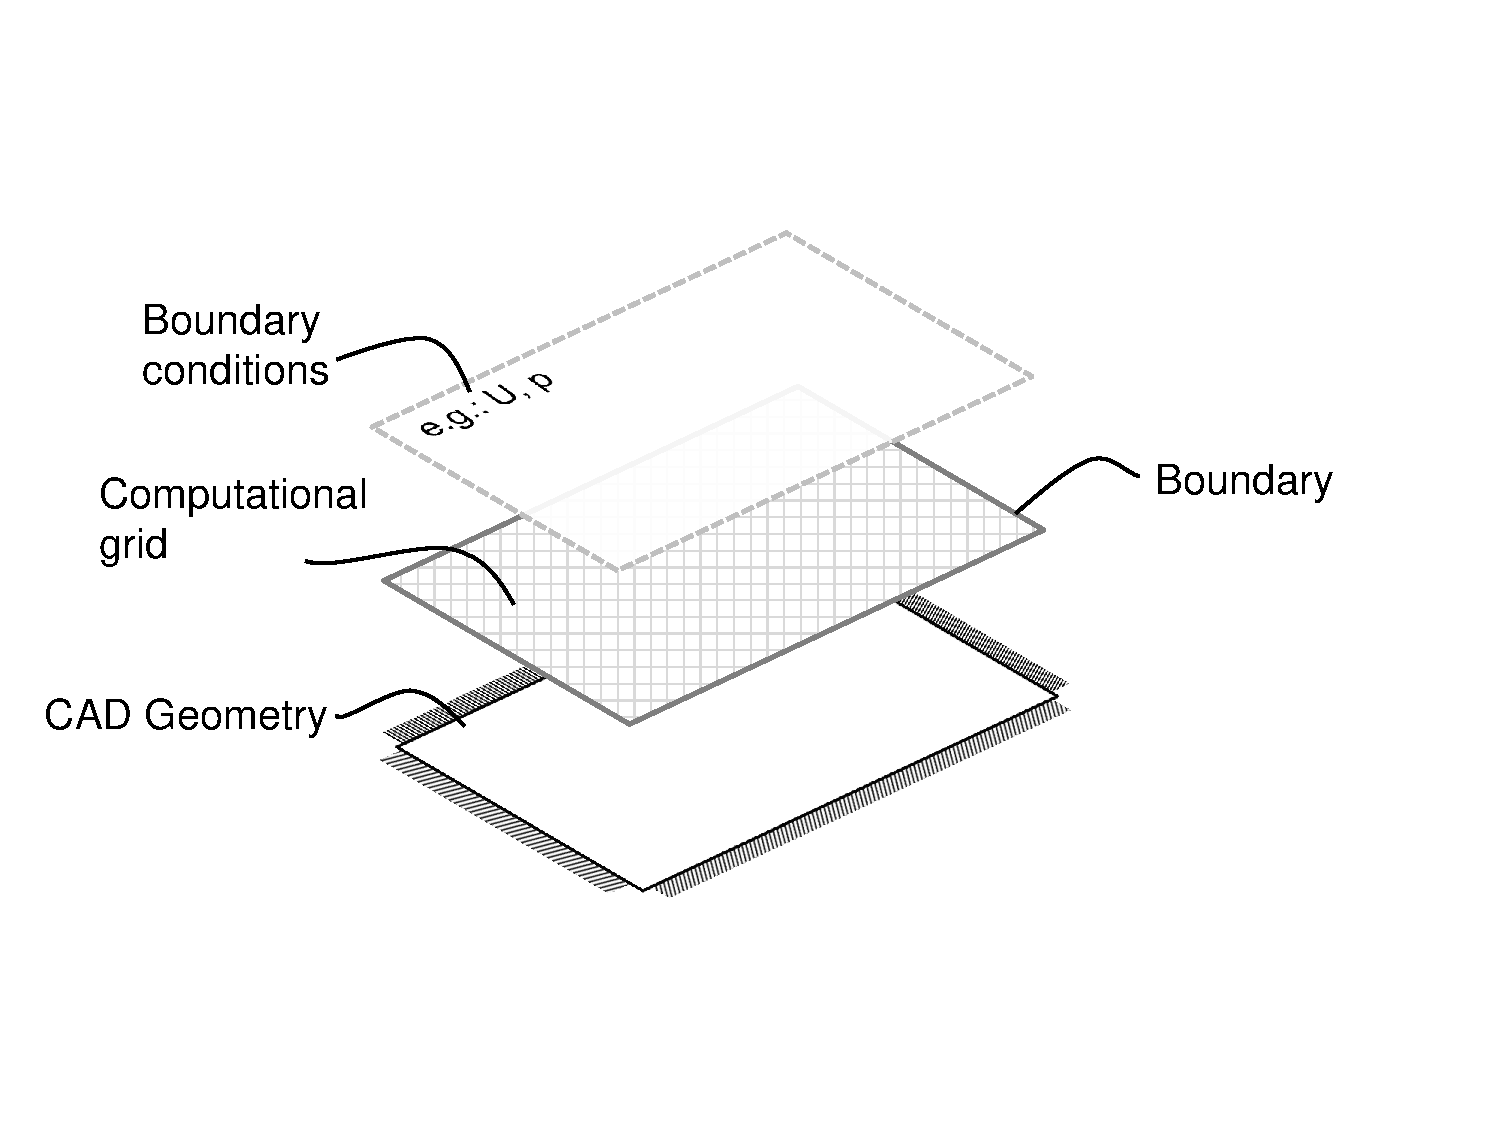
\includegraphics[width=0.6\linewidth, trim= 0cm 1cm 1cm 0, clip]{images/CAD_boundary}
	\captionsetup{format=plain,labelsep=newline}
	\caption[Relation between \gls{CAD} geometry, computational grid and boundary conditions]{Illustration of the relation between a \gls{CAD} geometry, the computational grid and its boundaries, and the boundary conditions applied. Adapted from \citep{Maric2014}.}
	\label{fig:cadboundary}
\end{sidefigure}

\item Before the simulation starts, physically appropriate boundary conditions as well as numerical settings have to be specified. The simulation eventually solves the algebraic set of equations by a solver that is tailored to capture the physical problem. The simulation ends after the simulation has reached either the final number of iterations or the specified convergence criteria.


\item Finally, the variables of interest need to be post-processed by visualizing the fluid flow with appropriate plots or further calculations. This should be supplemented by a verification/validation study in which the simulation is compared against measured values. An error estimation and sensibility analysis is needed to finally discuss the results. \CFD\ studies are usually of an iterative nature, which means the conclusions drawn will influence the pre-processing of the following simulation. This will procedure will be repeated until results are compliant with verification \& validation guidelines.

\end{enumerate}




\begin{figure}[htb]
	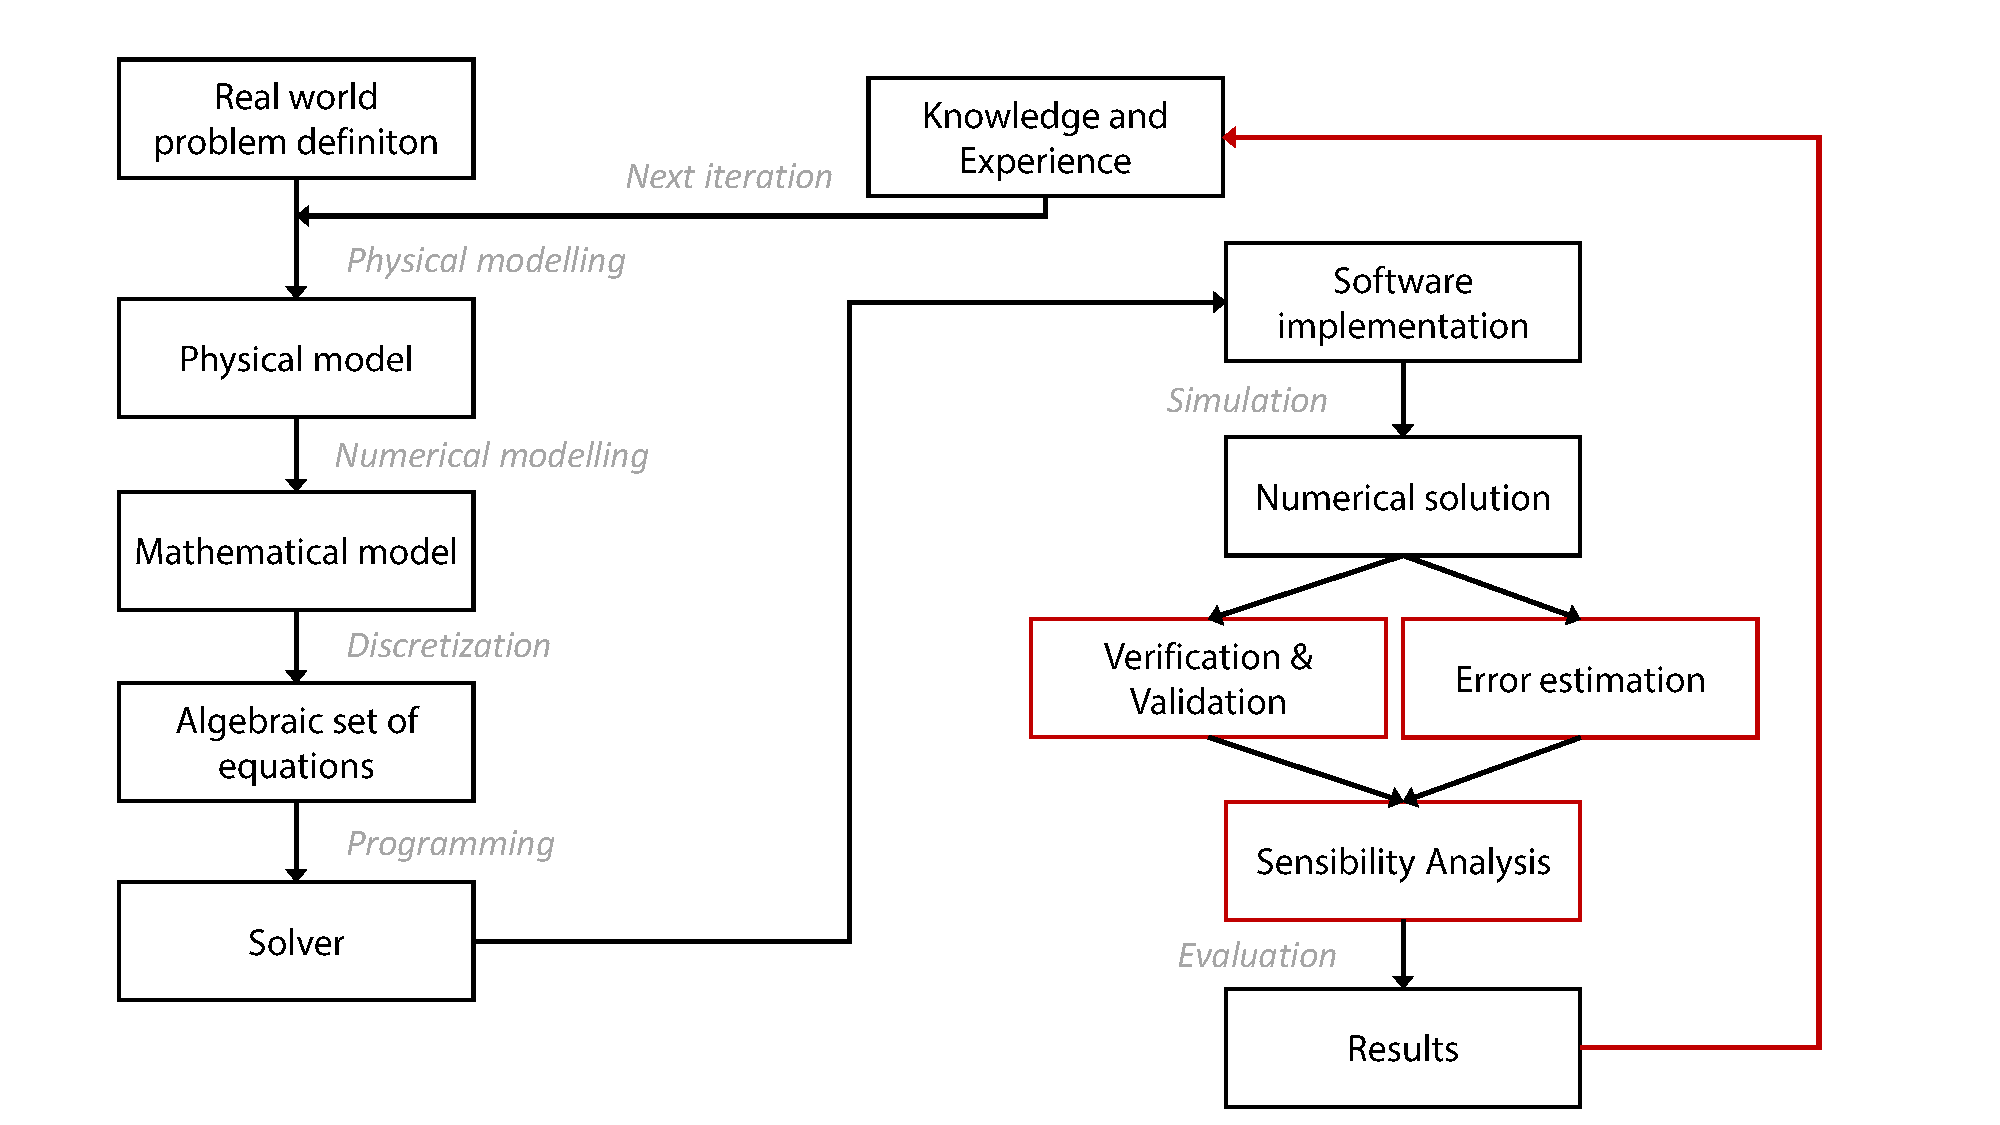
\includegraphics[width=1\linewidth, trim=1.1cm 0cm 1.1cm 0, clip]{images/cfd_schematic}
	\caption[Work-flow schematic for \CFD]{Work-flow schematic for \CFD. Adapted from \citep{Giglmaier2016}.}
	\label{fig:schema_cfd}
\end{figure}



%
% %
% % %
% % % %
% % %
% %
%

\clearpage
\section{Governing equations}
\label{sec:CFD:governing_equations}
\index{CFD!governing equations}

The \glsplural{NSE} describe the conservation of (1) mass , (2) momentum  and (3) energy.
The \glsplural{NSE} are derived from (1) the continuity equation, (2) Newton's second law and (3) the first law of thermodynamics. 
These equations treat the flow as a continuum and can be solved analytically only for several specific cases.
It is, however, possible to discretize the equations and solve them with regard to time and space.
The following notations $u$, $\bar{u}$, $u^{\prime}$ denote the instantaneous, mean, and fluctuating terms, respectively.

The continuity equation, also referred to as mass balance, is defined as:

\begin{equation}
\frac{\delta }{\delta t}\rho +\nabla (\rho \vec{u})= 0
\label{eq:theory:continuity}
\end{equation}

For a steady flow through a control volume, this equation shows that the net mass flux in the control volume must be zero.
The equation for linear momentum conservation, also know as the \gls{NSE} in its non-conservative form, is defined as:

\begin{equation}
\rho\left[\frac{\delta \vec{u}}{\delta t}+(\vec{u}\cdot\nabla)\vec{u} \right ]=-\nabla p + \nabla \bar{\bar{\tau}}+\rho \vec{f}
\label{eq:theory:momentum_conservation}
\end{equation}

where $\vec{f}$ is the body force per unit mass. If the weight of the fluid happens to be the only force present, $\vec{f}$ may be replaced with the gravitational vector $\vec{g}$.
$\bar{\bar{\tau}}$ is the symmetrical viscous stress tensor. For Newtonian fluids it is defined as:




\begin{equation}
\tau_{ij} = \mu \left(\frac{\delta u_i}{\delta x_j} +\frac{\delta u_j}{\delta x_i}\right )-\frac{2}{3} (\nabla \vec{u})\delta_{ij} ,\quad i,j = 1,2,3
\label{eq:CFD:stress_tensor}
\end{equation}


where $\delta_{ij}$ is the Kronecker-Delta operator, and \gls{symb:mu} is the \glsdesc{symb:mu} \citep{Sert2012}.

\paragraph*{Incompressible flows}
\index{CFD!incompressible flows}


For incompressible flows, density is defined as a constant, which leads to a simplified set of equations. Consequently,  \fref{eq:theory:continuity} reduces to:


\begin{equation}
\nabla \vec{u} = 0
\label{eq:CFD:continuity_imcompressible}
\end{equation}

\Fref{eq:CFD:continuity_imcompressible} states that the velocity field for incompressible flows is divergence-free. For the conservation of momentum, using \fref{eq:CFD:continuity_imcompressible} in  \fref{eq:CFD:stress_tensor}  cancels the second term in the stress tensor. Moreover, if viscous effects are negligible, \fref{eq:theory:momentum_conservation} simplifies to:



\begin{equation}
\rho\left[\frac{\delta \vec{u}}{\delta t}+(\vec{u}\cdot\nabla)\vec{u} \right ]=-\nabla p + \mu \nabla^2 \vec{u} +\rho \vec{f}
\label{eq:Navier_incompressible}
\end{equation}

\glsdesc{symb:mu} and \glsdesc{symb:nu} are related by the density.

\begin{equation}
\nu= \frac{\mu}{\rho}
\end{equation}

Thus, if we normalize \fref{eq:Navier_incompressible} by the density, we obtain the form of the \gls{NSE} that is commonly referred to when using this method.

\begin{equation}
\frac{\delta \vec{u}}{\delta t}+\underbrace{(\vec{u}\cdot\nabla)\vec{u}}_{\text{convective term}} =-\frac{1}{\rho}\nabla p + \underbrace{\nu \nabla^2 \vec{u}}_{\text{diffusion term}}+\vec{f}
\end{equation}


\gls{symb:nu} is the \glsdesc{symb:nu}, which is considered to be constant. 

In a 3-dimensional space, this yields \num{4} equations with \num{4} unknowns, namely the pressure and \num{3} velocity components.

%\section{Finite volume method}

The process of representing differential equations as a set of algebraic equations with equivalent properties is called discretization. In OpenFOAM, this is done with an approach called \gls{FVM}. This is necessary to solve the equations numerically.
After setting the appropriate \BC, it can be expressed in a linear equation system of the form:


\begin{equation}
\underline{A}\, \vec{x} = \vec{b}
\end{equation}

where $\vec{x}$ is the vector of the variable of interest, $\underline{A}$ is the square matrix and $\vec{b}$ is the source vector \citep{Sert2012}.

%
% %
% % %
% % % %
% % %
% %
%
